\section{Einleitung}

\subsection{Motivation}
Im Alltag eines Frontend-Entwicklers, eines Mitarbeiters an einem Web-Projekt oder des Entwicklers für das grafische User Interface kommt es nicht selten vor, dass die Beschreibung der grafischen Elemente durch Cascading Stylesheets geschieht. Noch seltener sind diese Style Angaben fehlerfrei. Sei es aufgrund von Zeitdruck, unterschiedlichen Entwicklern oder durch nachträgliches Bugfixing, oft sind CSS-Regeln inkonstistent aufgestellt, zum Beispieln existieren noch Regeln, die garnicht mehr im DOM der Seite zu finden sind. Es werden Regeln mehrmals überschrieben und es wird nicht auf Optimierung von Selektoren geachtet. 

% TODO: footnote mit link 
Seit 2010 berücksichtigt der Page Ranking Algorithmus von Google auch die Ladezeiten für Websites\footnote{Offizieller Blogpost: http://googlewebmastercentral.blogspot.de/2010/04/using-site-speed-in-web-search-ranking.html}. Seiten, die neben SEO\footnote{SEO: Search Engine Optimization / Suchmaschinenoptimierung} ein gutes Page Ranking erhalten, werden demnach auch durch ihre Ladezeiten bestimmt. Die Ladezeiten spielen zwar im Vergleich mit SEO nur eine kleine Rolle, können aber zu einem besseren Ergebnis beitragen (Weite Informationen: http://googlewebmastercentral.blogspot.de/2010/04/using-site-speed-in-web-search-ranking.html).
Ladezeiten von mobilen Websites und Web-Anwendungen bzw. Seiten, die über mobile Internetverbindungen geladen werden, sollten schnell und nur wenig Daten übertragen, um ein konsistentes Benutzererlebnis zu gewährleisten. Statistiken zeigen, dass Benutzer auf Websites eher verbleiben wenn diese schnell geladen werden und der Benutzer schnell Informationen abrufen oder mit der Anwendung interagieren kann.

\subsection{Anforderungen}

Im Rahmen der Hausarbeit für das Fach Compilerbau im Sommersemester 2013 im Master-Studiengang Informatik - Verteilte und Mobile Anwendungen an der Hochschule Osnabrück / University of Applied Sciences soll ein Werkzeug entwickelt werden mit dem sich Stylesheets optimieren lassen. Dazu soll ein Kommandozeilentool entwickelt werden, womit CSS-Optimierungen gesteuert und ausgegeben werden können. Nachfolgend werden die Anforderungen beschrieben.

\begin{description}
    \item[Ausgabeformat] Das Ausgabeformat soll ebenfalls als CSS-Datei geschrieben werden.
    
    \item[Ungenutztes CSS entfernen] Deklarierte Regeln die in HTML-Dateien nicht eingesetzt werden, sollen entfernt werden, da sie überflüssig sind.
    
    \item[Gleiche CSS-Regeln zusammenführen] Selektoren
    
    \item[Shorthands für Hex-Farbwerte] 
    
    \item[]
\end{description}

\subsection{Konzeption}

% TODO: check reference numbering
Die vorgestellten Anforderungen an den CSS-Optimierer werden in der Abbildung \ref{app-workflow} als Flow-Diagram beschrieben. 
 
% TODO: flow diagram überarbeiten
\begin{figure}[h!]
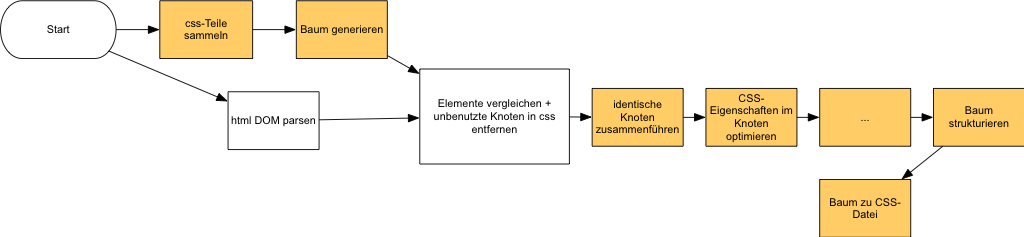
\includegraphics[width=1.0\textwidth]{img/app-workflow.png}
\label{app-workflow}
\end{figure}

\begin{description}
    \item[CSS-Datein sammeln]

    \item[Baum generieren]
    
    \item[ungenutzte Knoten entfernen]
    
    \item[merge same nodes]
    
    \item[CSS-Eigenschaften je node optimieren]
    
    \item[Restrukturierung des Baums]
    
    \item[Baum zu CSS]    
\end{description}

